\chapter{Contexte Général}

\section{Introduction}

Ce chapitre pose le cadre institutionnel du projet en présentant la structure d’accueil au sein de laquelle le travail a été effectué. L'étude débute par un historique et une vue d'ensemble des missions stratégiques de l'entreprise nationale en charge de l'énergie, avant de détailler l'organisation technique de la direction régionale de rattachement. Cette immersion permet de mieux appréhender les flux opérationnels existants et de situer l'application développée dans son environnement organisationnel réel.

\section{STEG}

\subsection{Présentation de la société}

À la veille de l'indépendance de la Tunisie, l'activité électrique nationale était fragmentée et gérée par sept sociétés concessionnaires distinctes. Ces structures assuraient l'alimentation des principales régions du pays avec une puissance totale installée de près de 100 MW pour une production annuelle d'environ 240 GWh. 

Dans le but d'harmoniser, de centraliser et d'optimiser le secteur de l'énergie stratégique, l'État tunisien a promulgué la loi numéro 62-8 du 3 avril 1962, portant création de la Société Tunisienne de l'Électricité et du Gaz. Cette institution s'est vu confier le monopole de la production, du transport et de la distribution de l'électricité ainsi que du gaz sur l'ensemble du territoire national.

Les missions fondamentales assignées à l'entreprise s'articulent autour de l'électrification globale du pays, de l'extension progressive du réseau de gaz naturel et de la réalisation d'infrastructures d'envergure. À ce titre, la structure assure la responsabilité technique et commerciale de l'approvisionement énergétique du marché national afin de répondre aux exigences croissantes des différents secteurs de consommation, qu'ils soient résidentiels, industriels ou tertiaires.

Sur le plan opérationnel, les activités couvrent la production de l'énergie électrique à partir de sources diversifiées telles que le thermique, l'hydraulique ou l'éolien, ainsi que la fabrication du Gaz de Pétrole Liquéfié. Le transit de cette énergie s'effectue via un réseau de transport composé de lignes et de postes à haute tension, relayé par un réseau de distribution à moyenne et basse tension assurant l'acheminement final auprès des usagers.

\subsection{Organigramme de la société}

\begin{figure}[H]
  \centering
  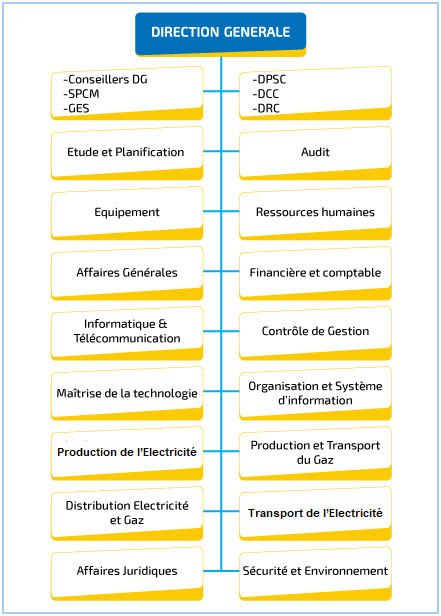
\includegraphics[width=0.9\textwidth]{../../assets/organigrammeSTEG.png}
  \caption{Organigramme général de la STEG} 
  \label{fig:organigrammeSTEG}
\end{figure}

\subsection{Département d'Exploitation Informatique Sud}

Le Département d'Exploitation Informatique Sud constitue l'entité technique pivot chargée de garantir la continuité, la sécurité et la performance des infrastructures informatiques pour les structures régionales. Ce service assure la supervision des systèmes de communication, l'administration des bases de données locales, ainsi que la maintenance du parc matériel et logiciel utilisé par les agents. C'est au sein de cet environnement technologique que s'est déroulée la conception de la solution, permettant d'aligner le développement de l'application sur les standards d'exploitation et les exigences de sécurité de la direction.

\subsection{Organigramme de la Département d'Exploitation Informatique Sud}

\begin{figure}[H]
  \centering
  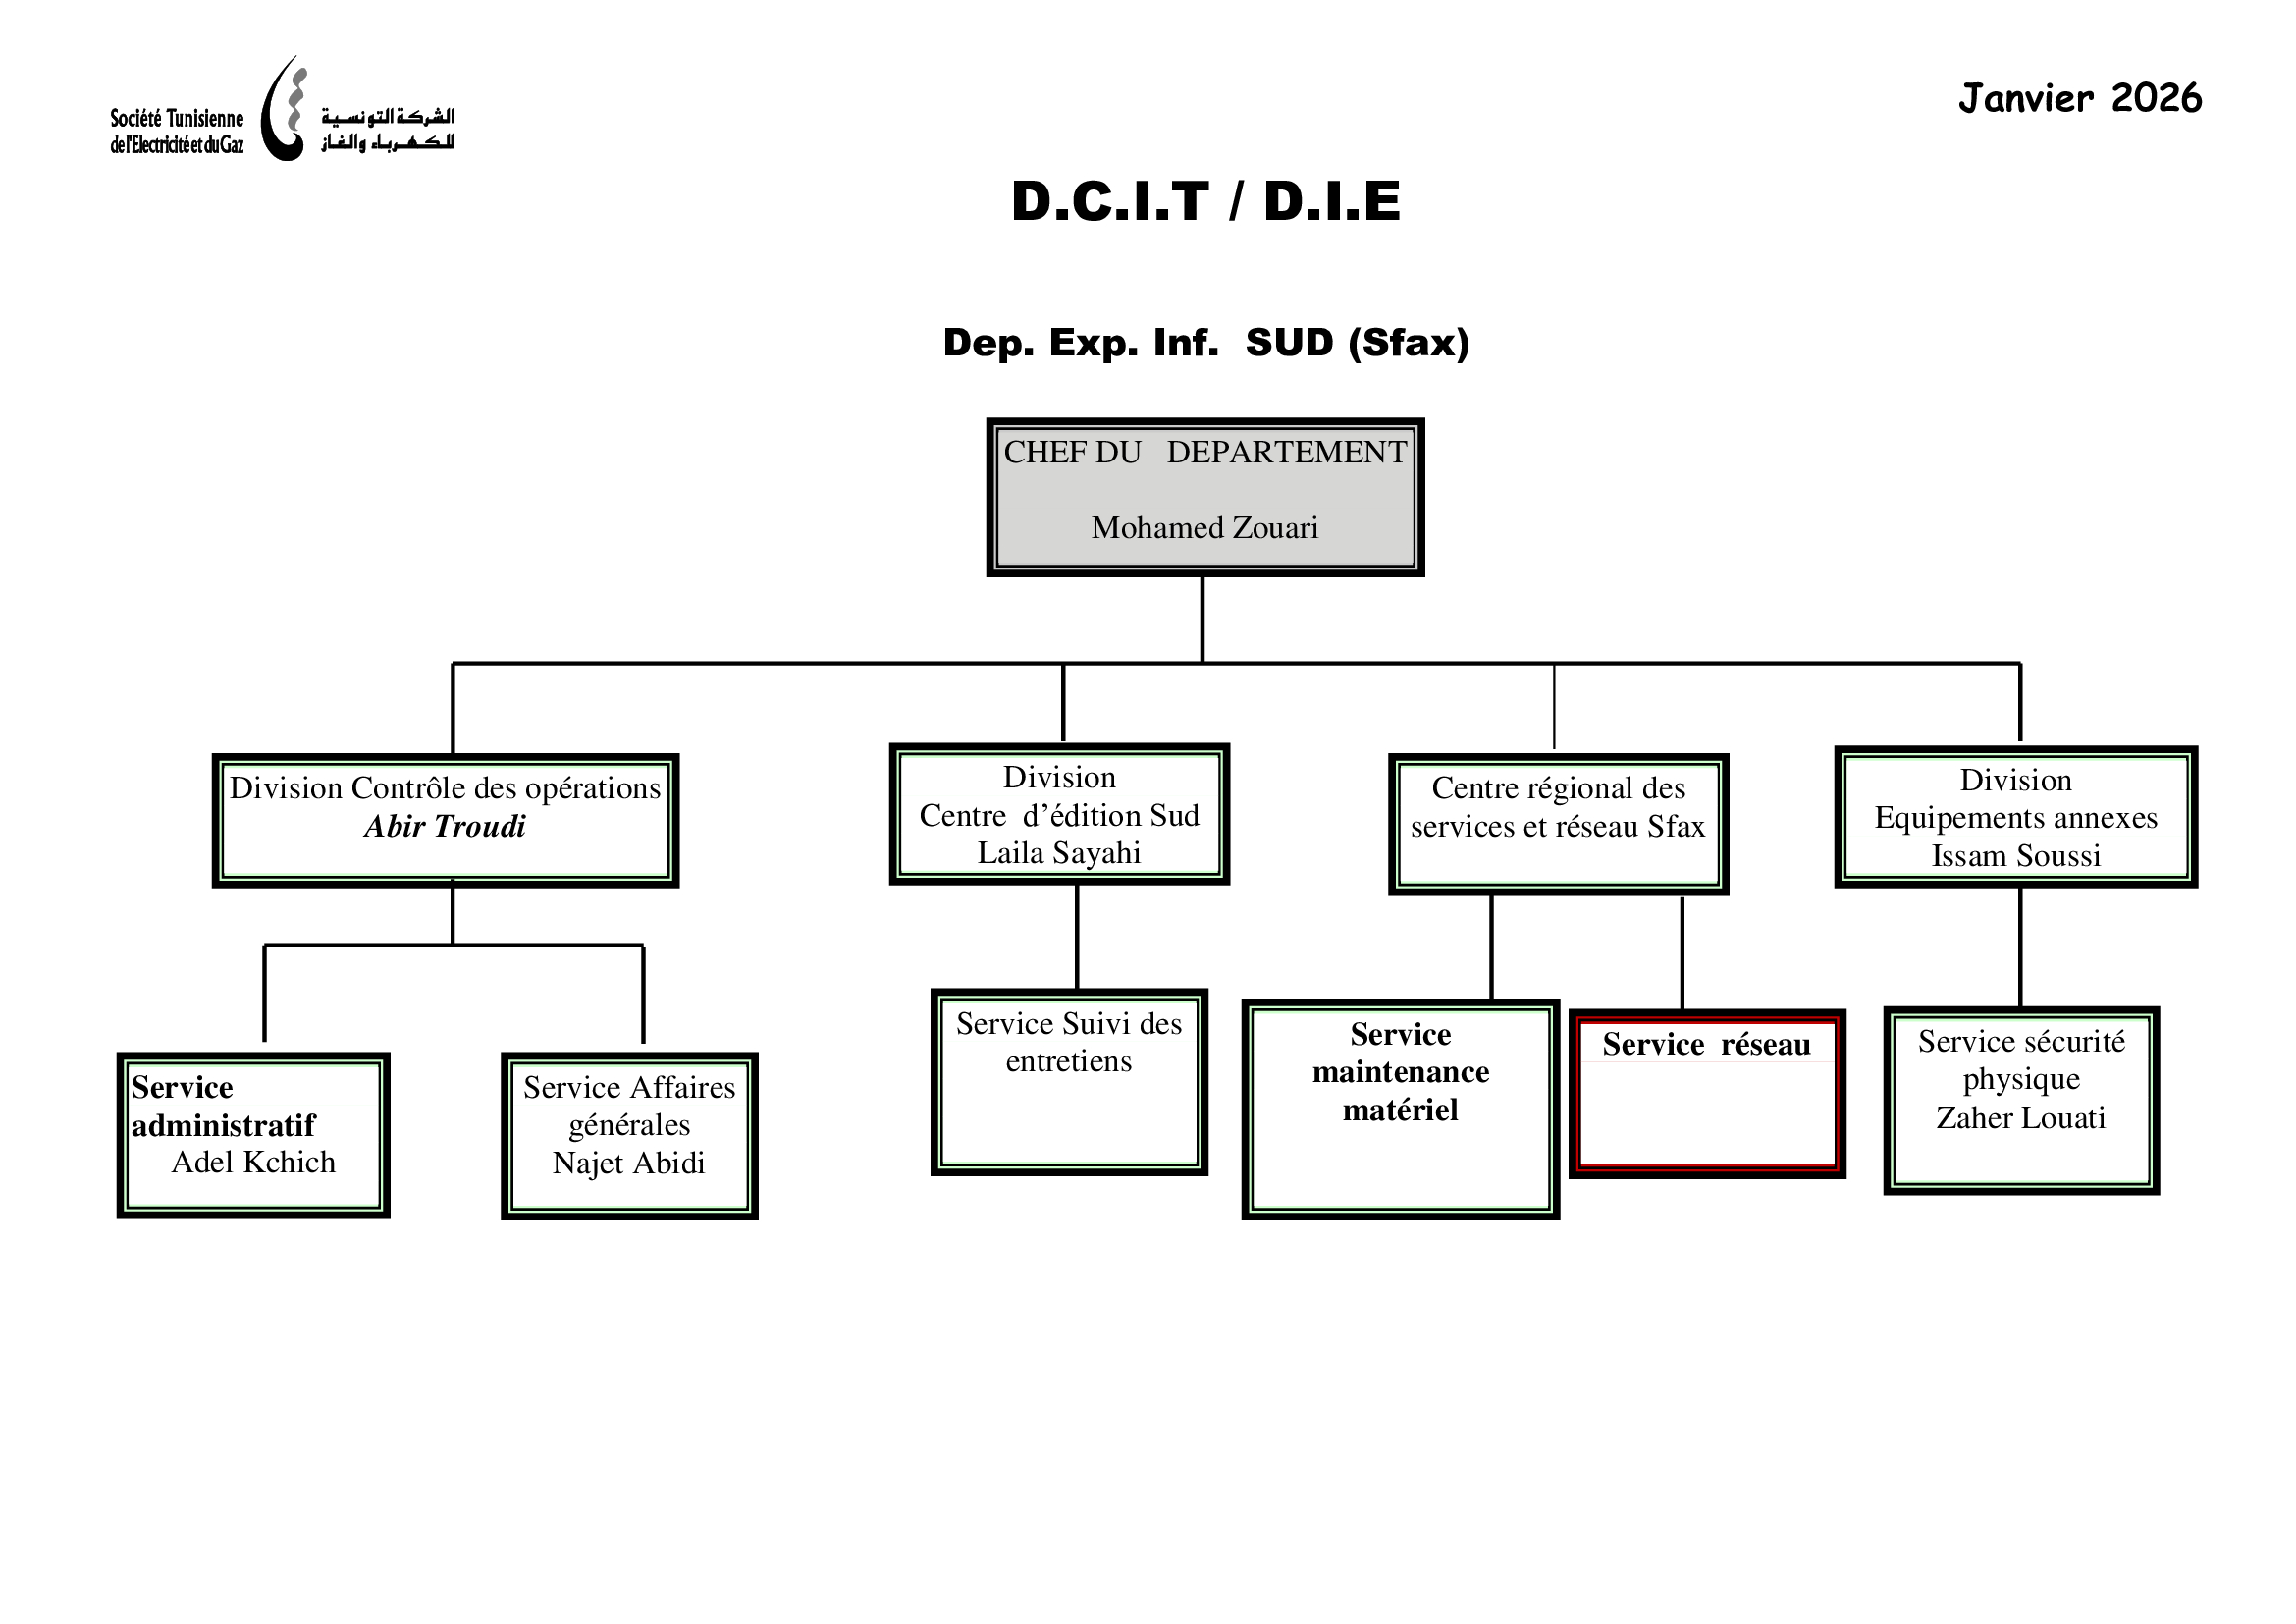
\includegraphics[width=0.9\textwidth]{../../assets/Organigramme-Dep-Exp-Sud.jpg}
  \caption{Organigramme général de la Département d'Exploitation Informatique Sud} 
  \label{fig:Organigramme-Dep-Exp-Sud}
\end{figure}